\documentclass{beamer}
\usepackage{amsmath, amsfonts, amssymb, amsthm}
\usepackage{graphicx, caption, hyperref, url, cite}
\usepackage[UTF8, noindent]{ctexcap}

\usetheme{Boadilla}
\usefonttheme[onlymath]{serif}

\title{0511汇报}
\institute{项目三}
\author{朱睿涵 \and 李宸亦}
\date{\today}

\setbeamertemplate{bibliography item}[text]

\begin{document}

\frame{\titlepage} % 标题页

\AtBeginSection{
    \begin{frame}
        \frametitle{目录}

        \tableofcontents[currentsection]
    \end{frame}
}

\section{基于多任务学习的生成式阅读理解}
\subsection{现有问题}
\begin{frame}
    \frametitle{现有问题}

    目前主流的机器阅读理解模型:抽取式

    \begin{itemize}
        \item 特点:将答案设定为段落中的一个连续片段
        \item 局限:不自然、不通顺
    \end{itemize}

    生成式 vs 抽取式:

    \begin{itemize}
        \item 生成式不再局限于直接从段落中抽取答案
        \item 参考段落、问题、词表生成答案
        \item 更完整、更自然、更流畅
    \end{itemize}

    现有生成式模型的问题:通常基于整个段落生成答案,\textbf{缺乏对答案边界和问题类型信息的理解}

    \begin{itemize}
        \item 本文的解决方案:基于多任务学习的生成式阅读理解框架
        \item 本文baseline模型:UniLMV2模型
    \end{itemize}

\end{frame}

\subsection{多任务学习}
\begin{frame}
    \frametitle{多任务学习}

    多任务学习机制:可提高模型泛化能力

    机制:

    \begin{itemize}
        \item 同时学习多个相关任务,让这些任务同时共享知识
        \item 利用任务之间的相关性,提升每个任务的泛化性能
    \end{itemize}

    一般做法:

    \begin{itemize}
        \item 在所有任务上共享模型编码层
        \item 针对特定的任务层有所区别
    \end{itemize}

    \begin{block}{本文模型的多任务}
        \begin{itemize}
            \item 答案生成(主任务)
            \item 答案抽取(辅助任务)
            \item 问题分类(辅助任务)
        \end{itemize}
    \end{block}

\end{frame}

\subsection{模型}
\begin{frame}
    \frametitle{模型概览}

    本文提出的生成式阅读理解模型由编码层和任务层组成:

    \begin{figure}
        \centering
        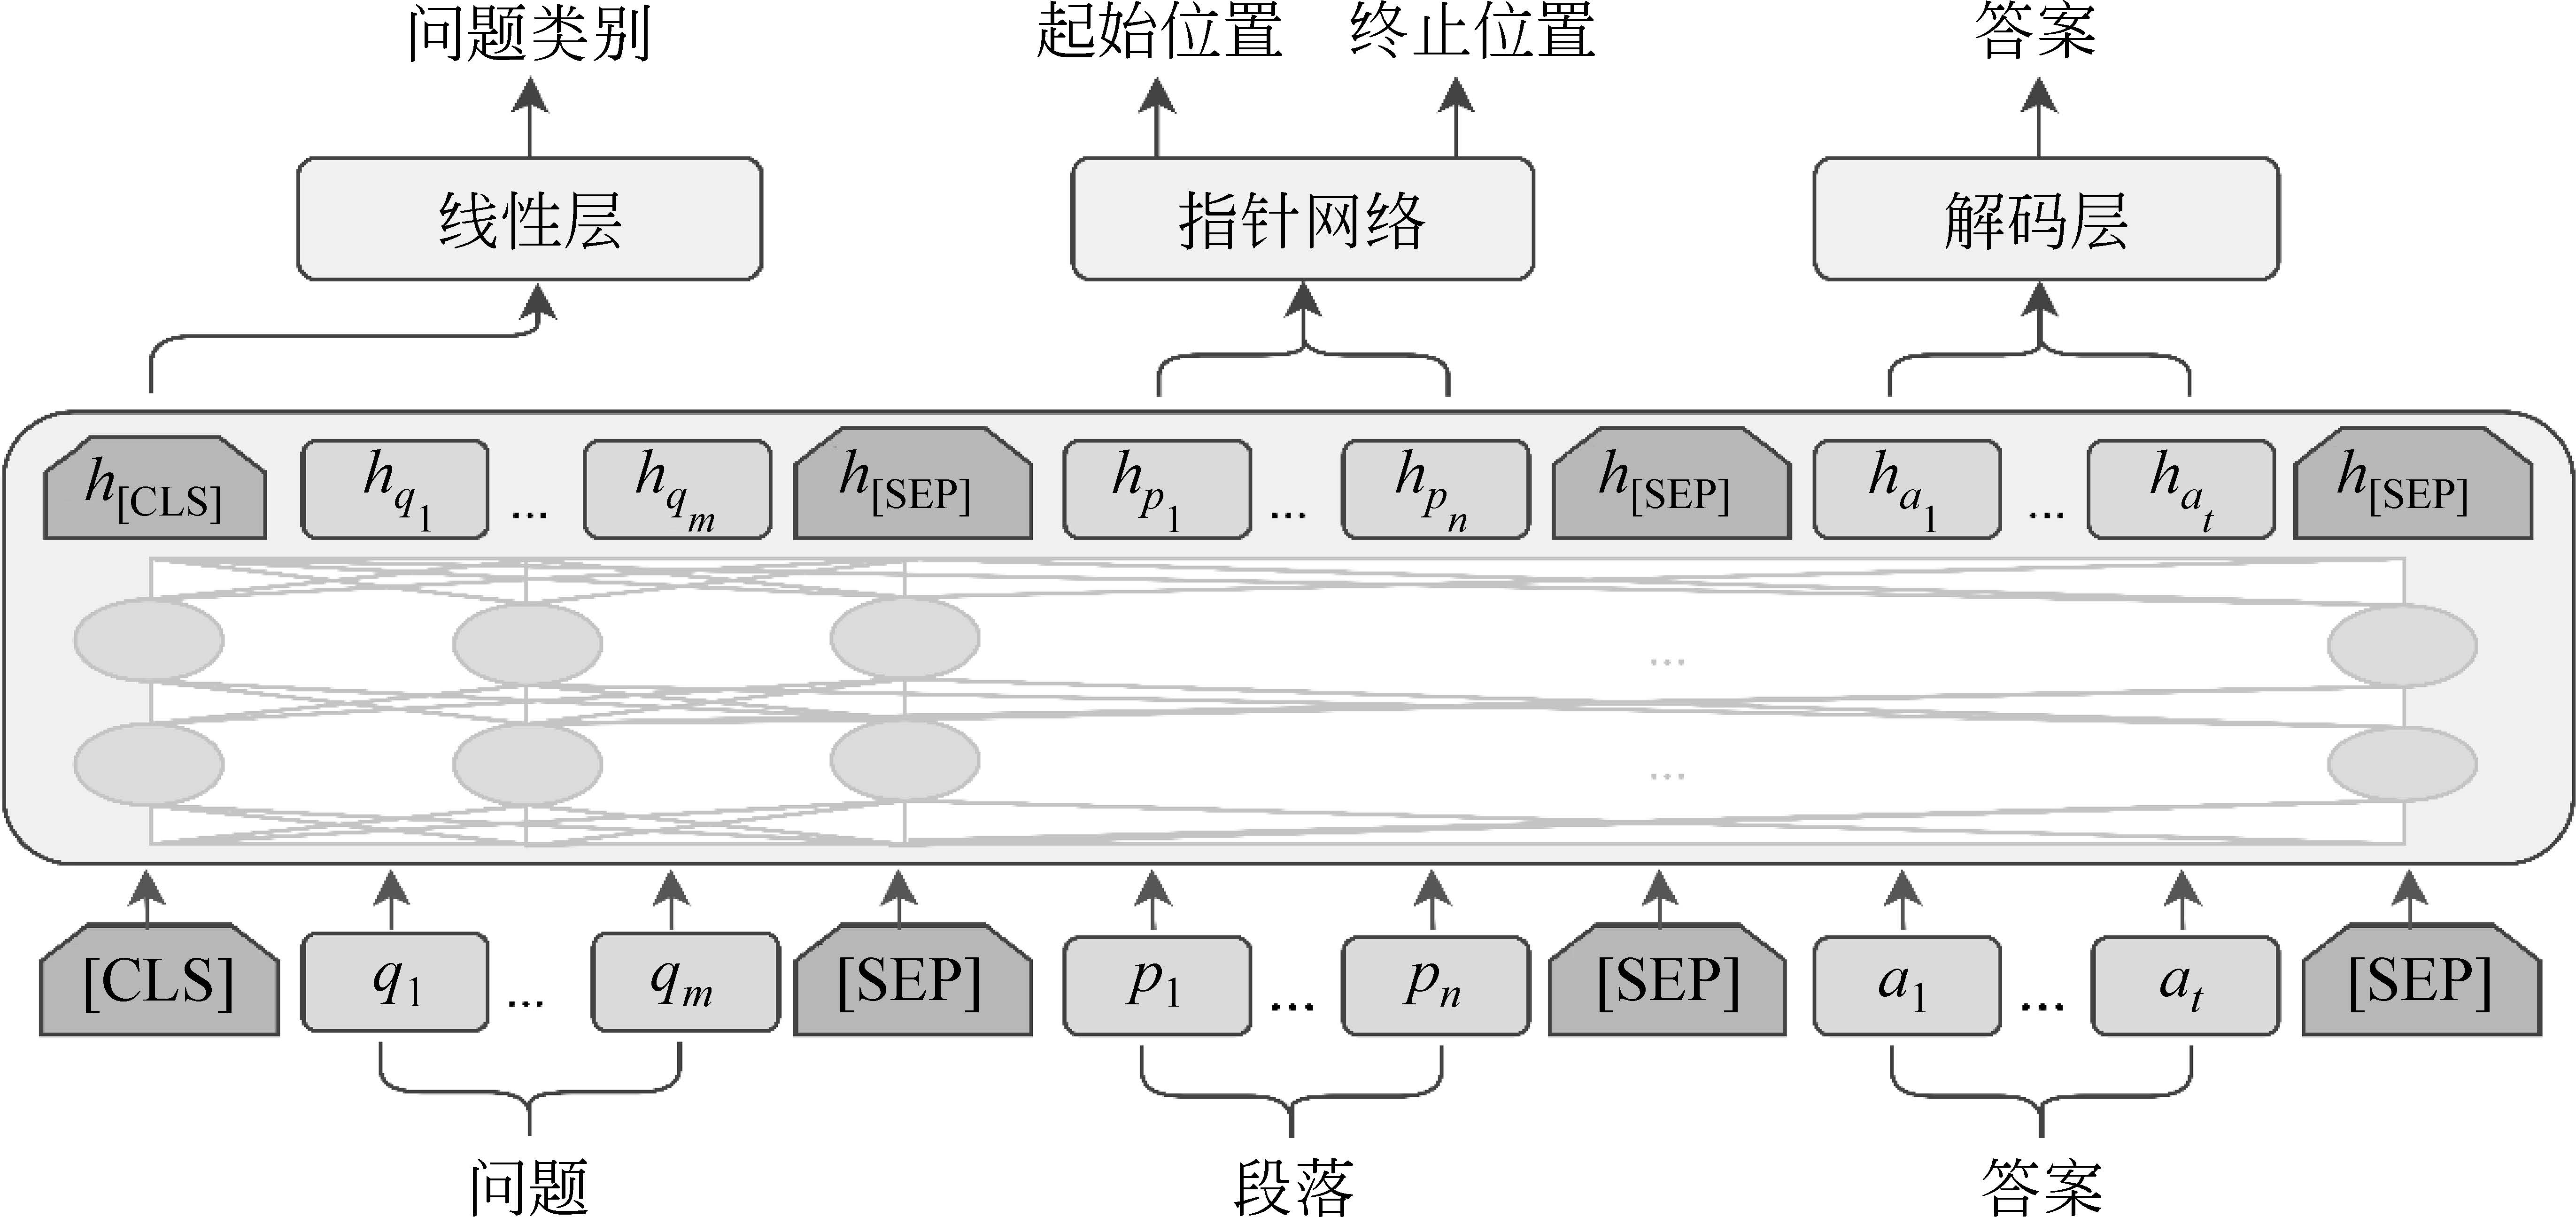
\includegraphics[width=0.6\textwidth]{./fig/model.jpg}
    \end{figure}

    \begin{itemize}
        \item 编码层:
        \begin{itemize}
            \item 基于深度双向Transformer编码器
            \item 借鉴UniLMV2的自注意力掩码机制控制答案生成过程中的可见信息
        \end{itemize}
        \item 任务层:
        \begin{itemize}
            \item 答案生成模型:beam search解码生成
            \item 答案抽取模型:指针网络识别答案位置
            \item 问题分类模型:线性层判断问题具体类型
        \end{itemize}
    \end{itemize}

\end{frame}

\subsubsection{编码层}
\begin{frame}
    \frametitle{编码层}

    \begin{figure}
        \centering
        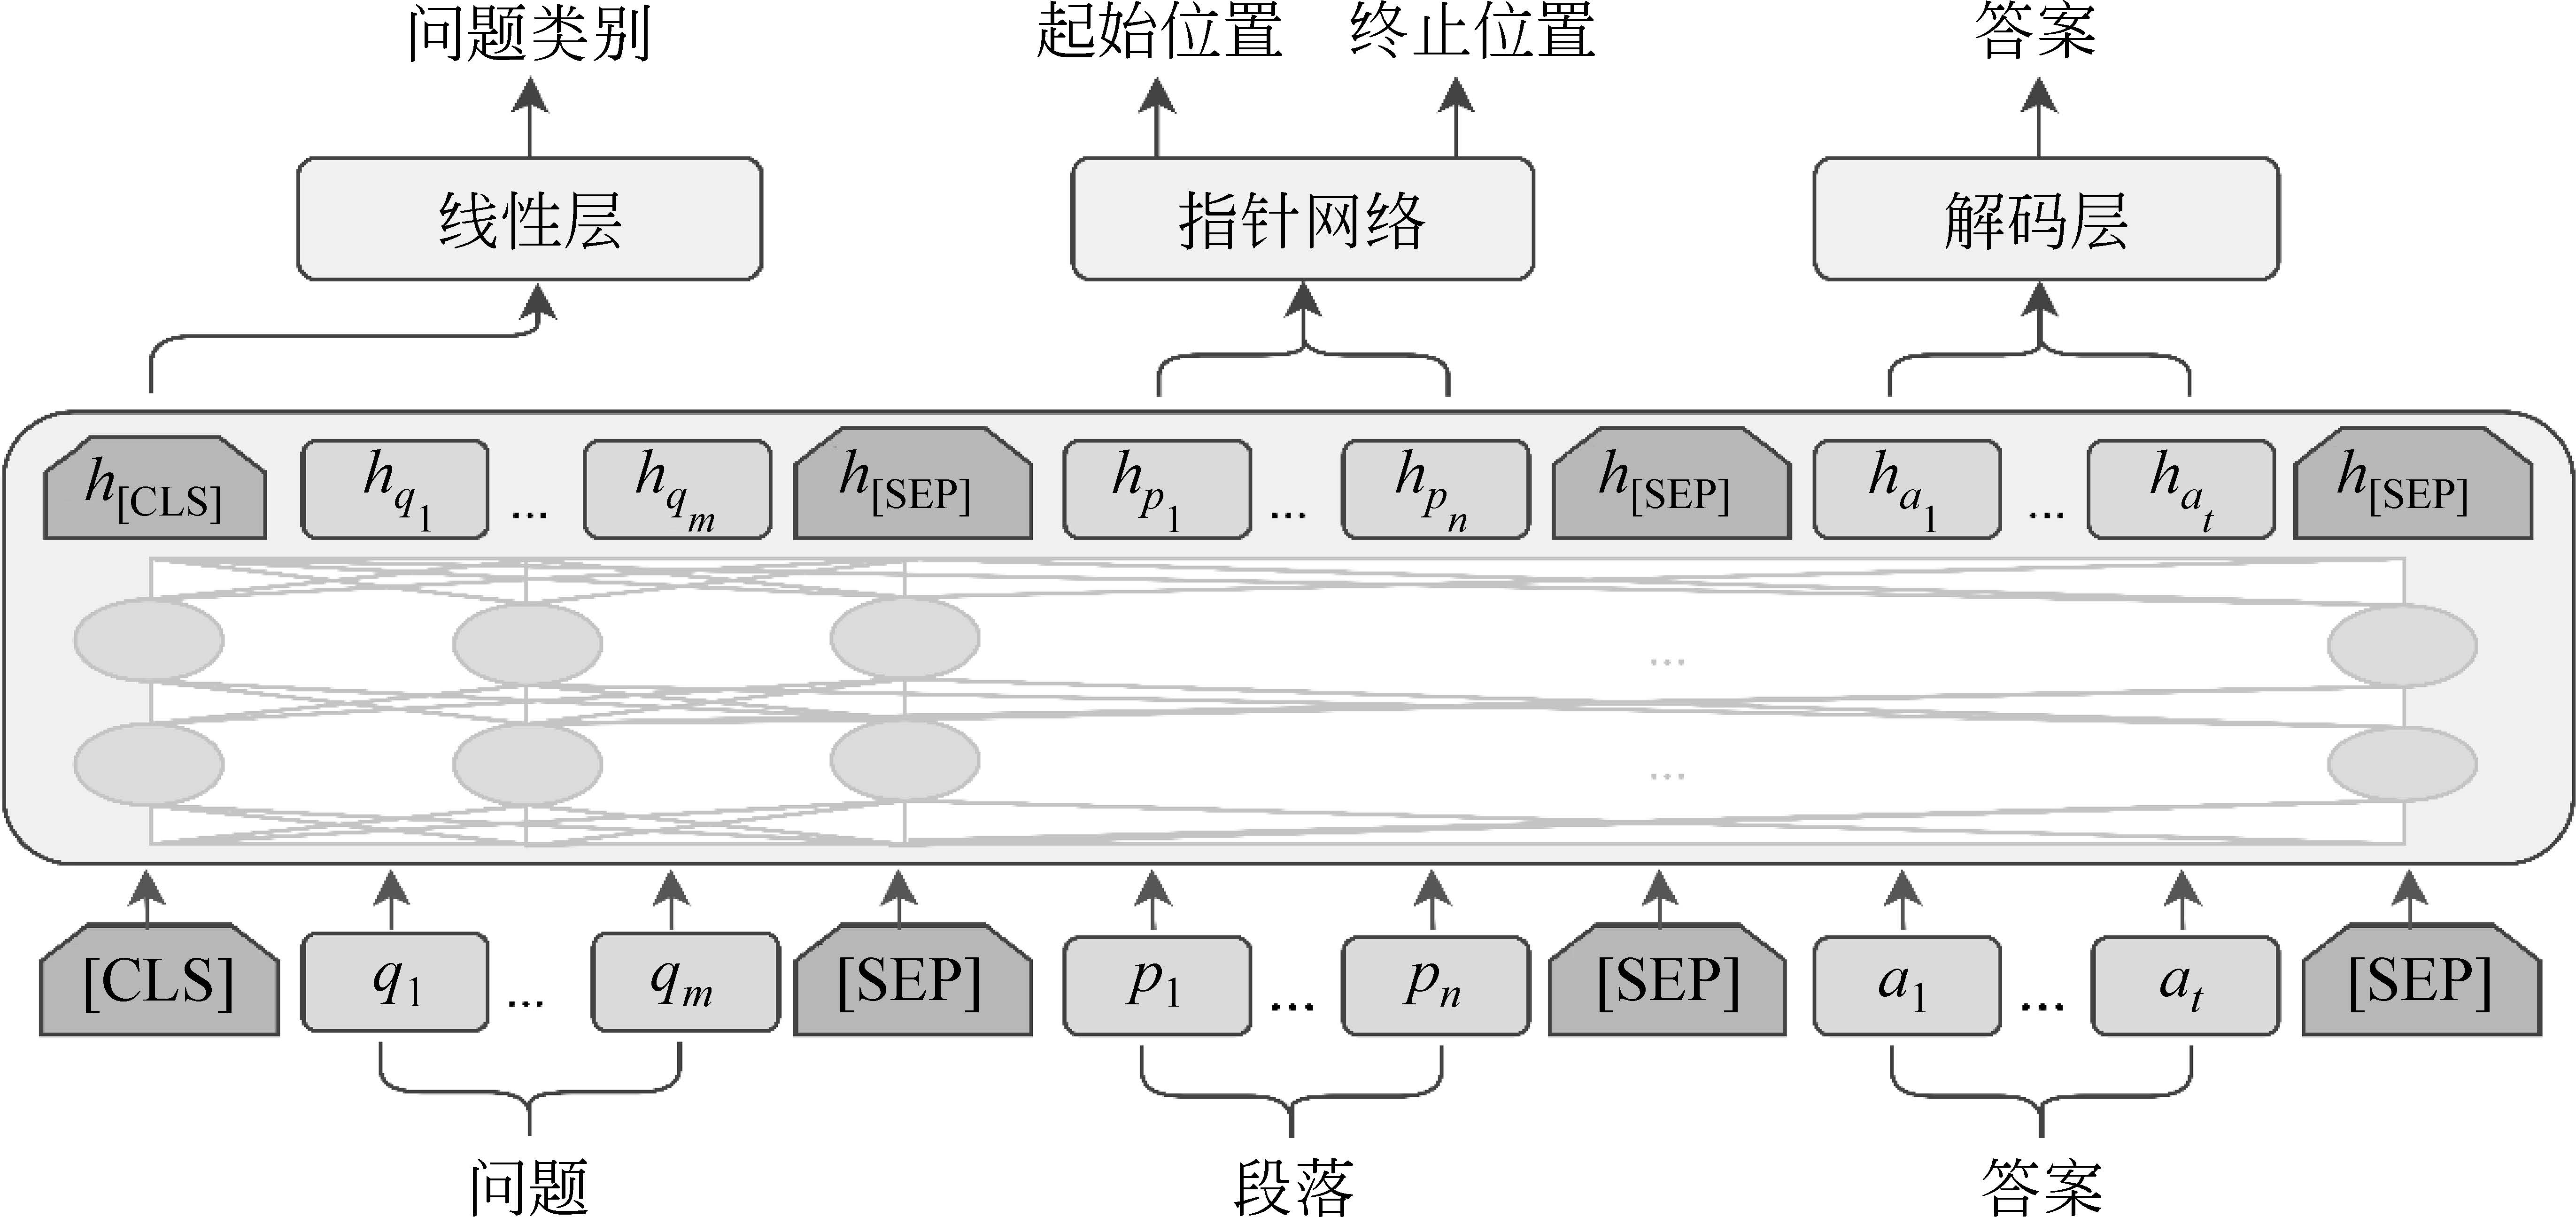
\includegraphics{./fig/model.jpg}
    \end{figure}

    \begin{itemize}
        \item 基于预训练模型UniLMV2构建编码层
        \item 采用预训练的BERT进行问题和段落的交互
        \item 改进注意力遮蔽矩阵,采用伪遮蔽语言模型
    \end{itemize}

\end{frame}

\begin{frame}
    \frametitle{编码层具体原理和过程}

    词嵌入:

    \begin{itemize}
        \item 采用WordPiece分词工具,将问题、段落和答案分词
        \item 对答案的部分词项进行一定概率的遮蔽,拼接后作为模型输入
        
        词向量$X_i$:
        \begin{equation}
            X_i = WE(w_i) + SE(w_i) + PE(w_i)
        \end{equation}

        输入序列表示为:
        \begin{equation}
            H^0 = [X_1, X_2, ..., X_{\lvert x \rvert}]
        \end{equation}
    \end{itemize}

    编码层:UniLMV2的编码层使用12层堆叠的Transformer网络
    
    \begin{itemize}
        \item Transformer两个子层:
        
        \begin{equation}
            LayerNorm(x + SubLayer(x))
        \end{equation}

        \begin{itemize}
            \item 多头注意力机制
            \item 前向神经网络
        \end{itemize}
    \end{itemize}

\end{frame}

\begin{frame}
    \frametitle{编码层具体原理和过程}

    Transformer的自注意力头$A_l$计算:

    \begin{equation}
        A_l = softmax(\frac{Q_l K_l^T}{\sqrt{d_k}} + M) V_l
    \end{equation}

    \begin{equation}
        Q_l = H^{l - 1} W_l^Q, K_l = H^{l - 1} W_l^K, V_l = H^{l - 1} W_l^V
    \end{equation}
\end{frame}

\begin{frame}
    \frametitle{编码层具体原理和过程}

    $M$为注意力遮蔽矩阵:

    \begin{figure}
        \centering
        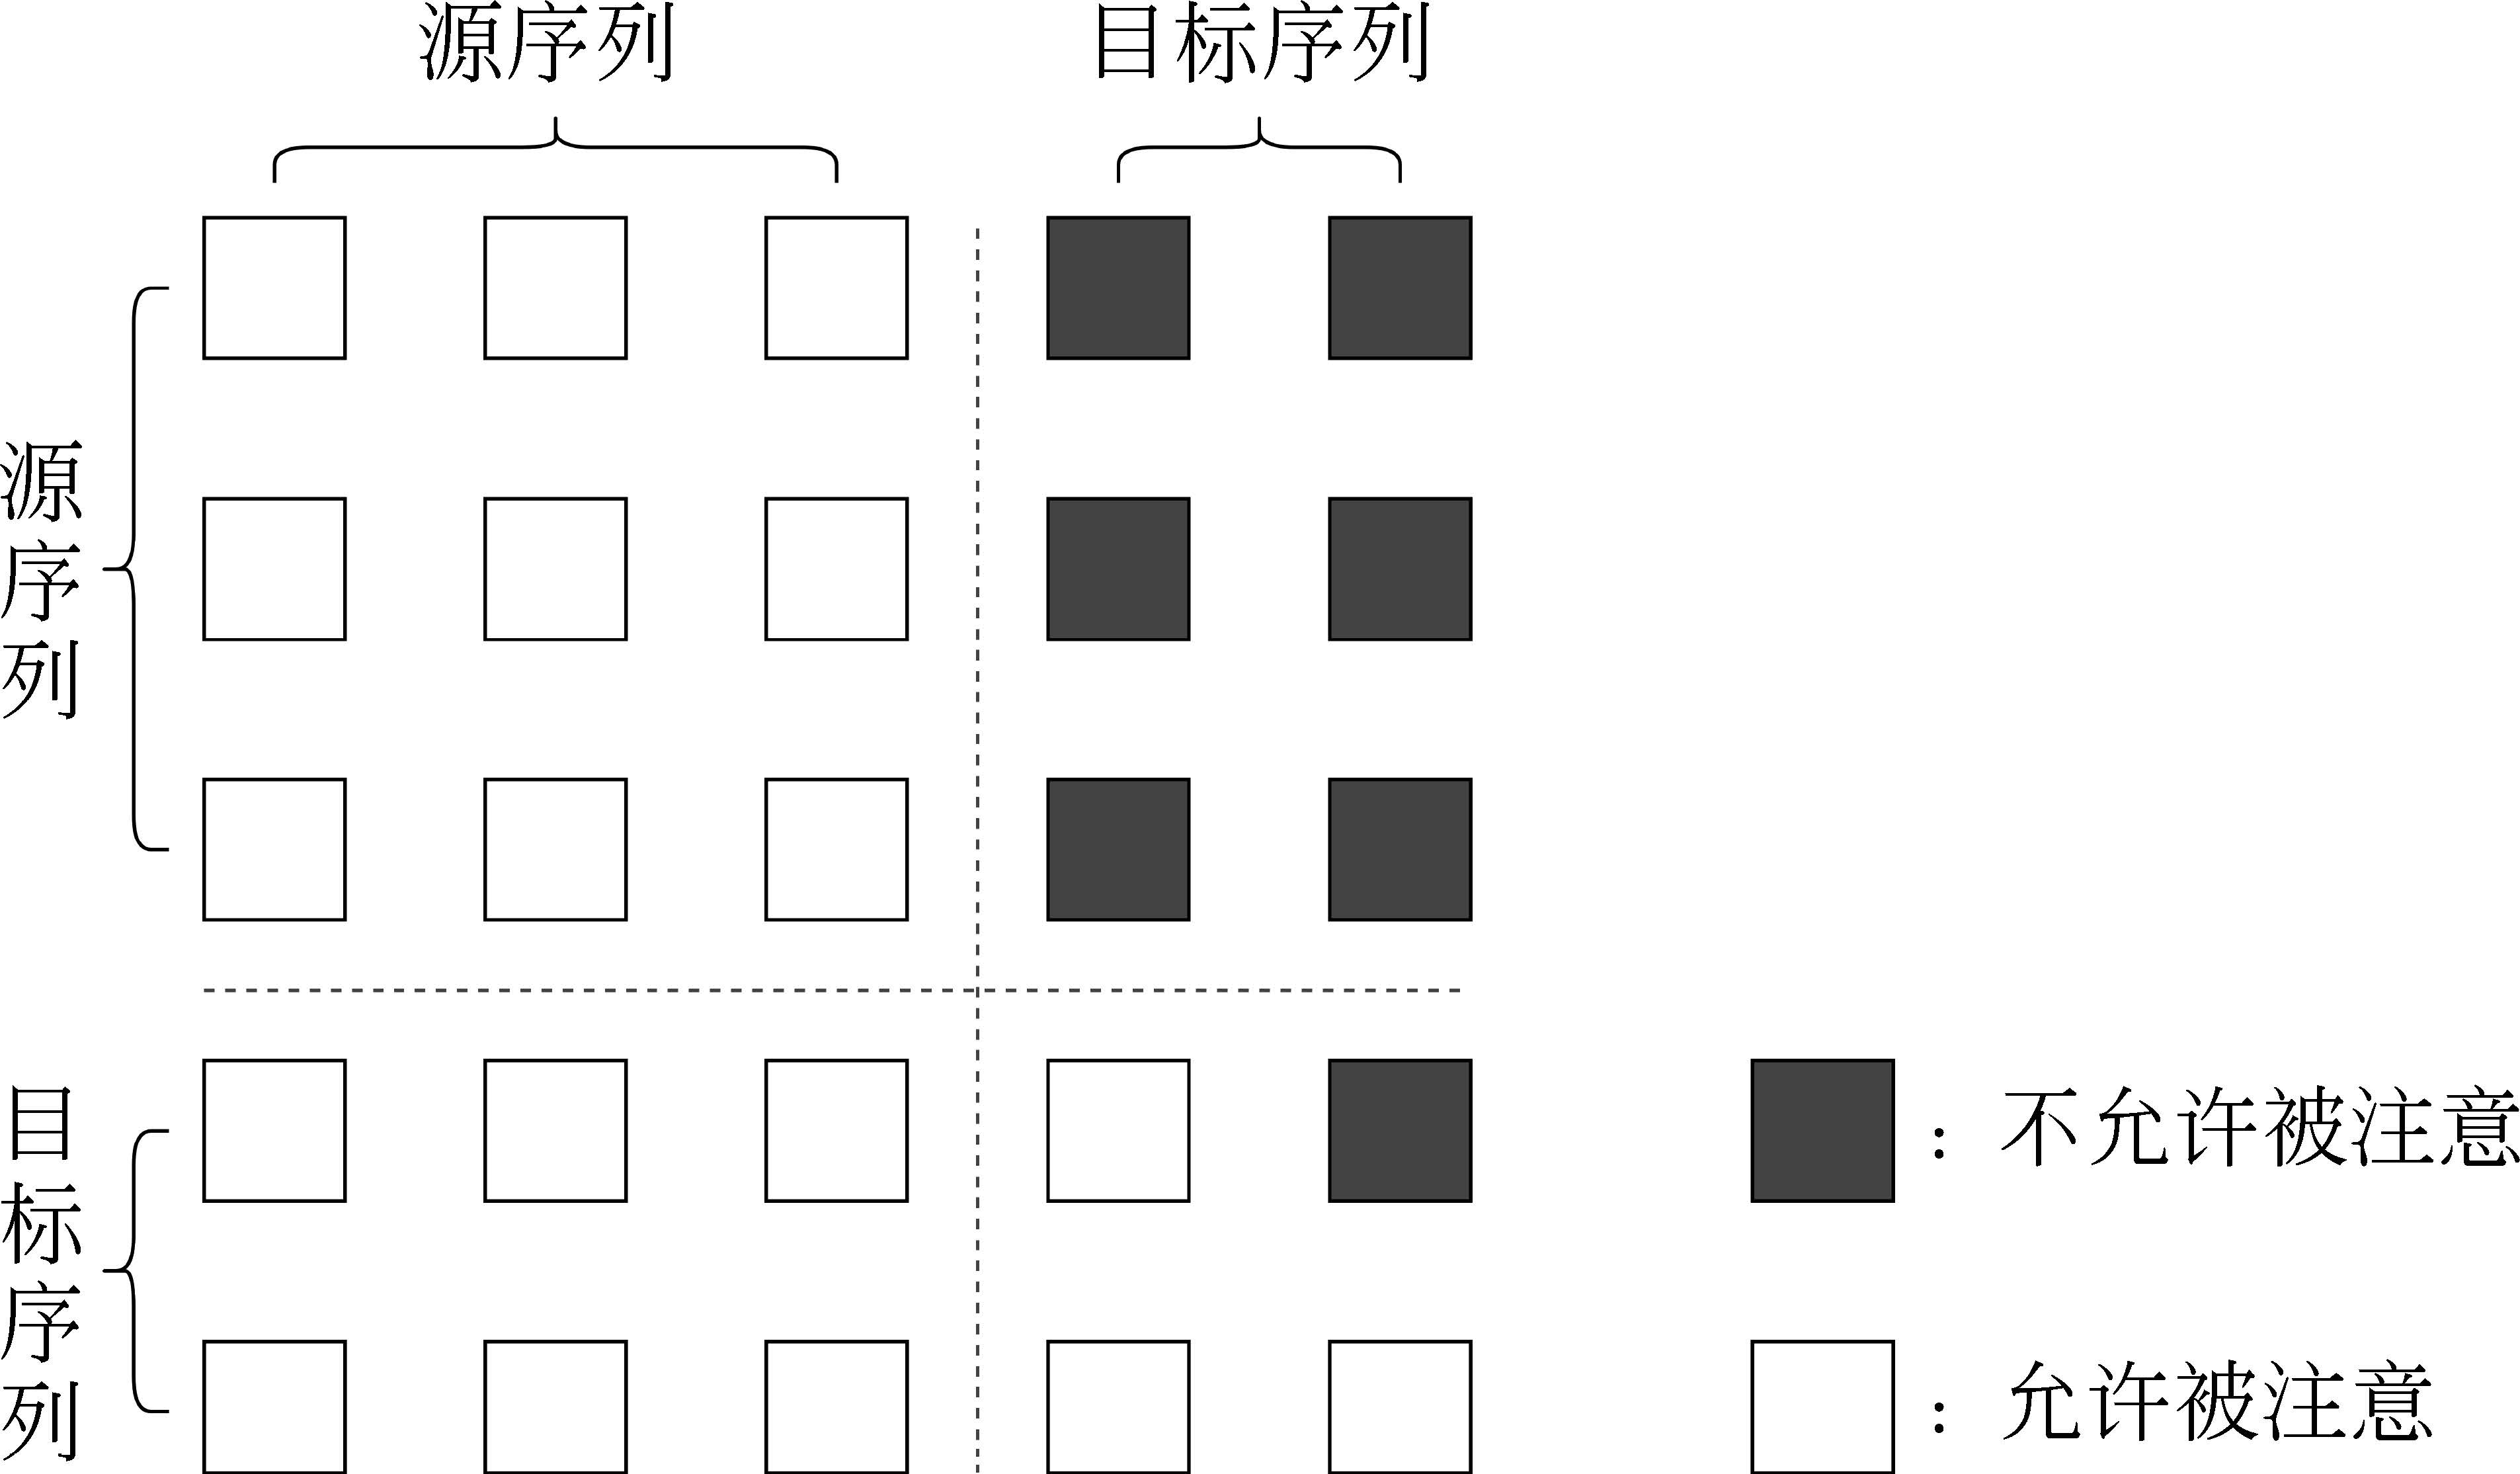
\includegraphics{./fig/mask.jpg}
    \end{figure}

    问题和段落不会和答案进行交互,保证了训练和测试阶段所含信息的一致性

\end{frame}

\subsubsection{任务层}
\begin{frame}
    \frametitle{任务层}

    \begin{figure}
        \centering
        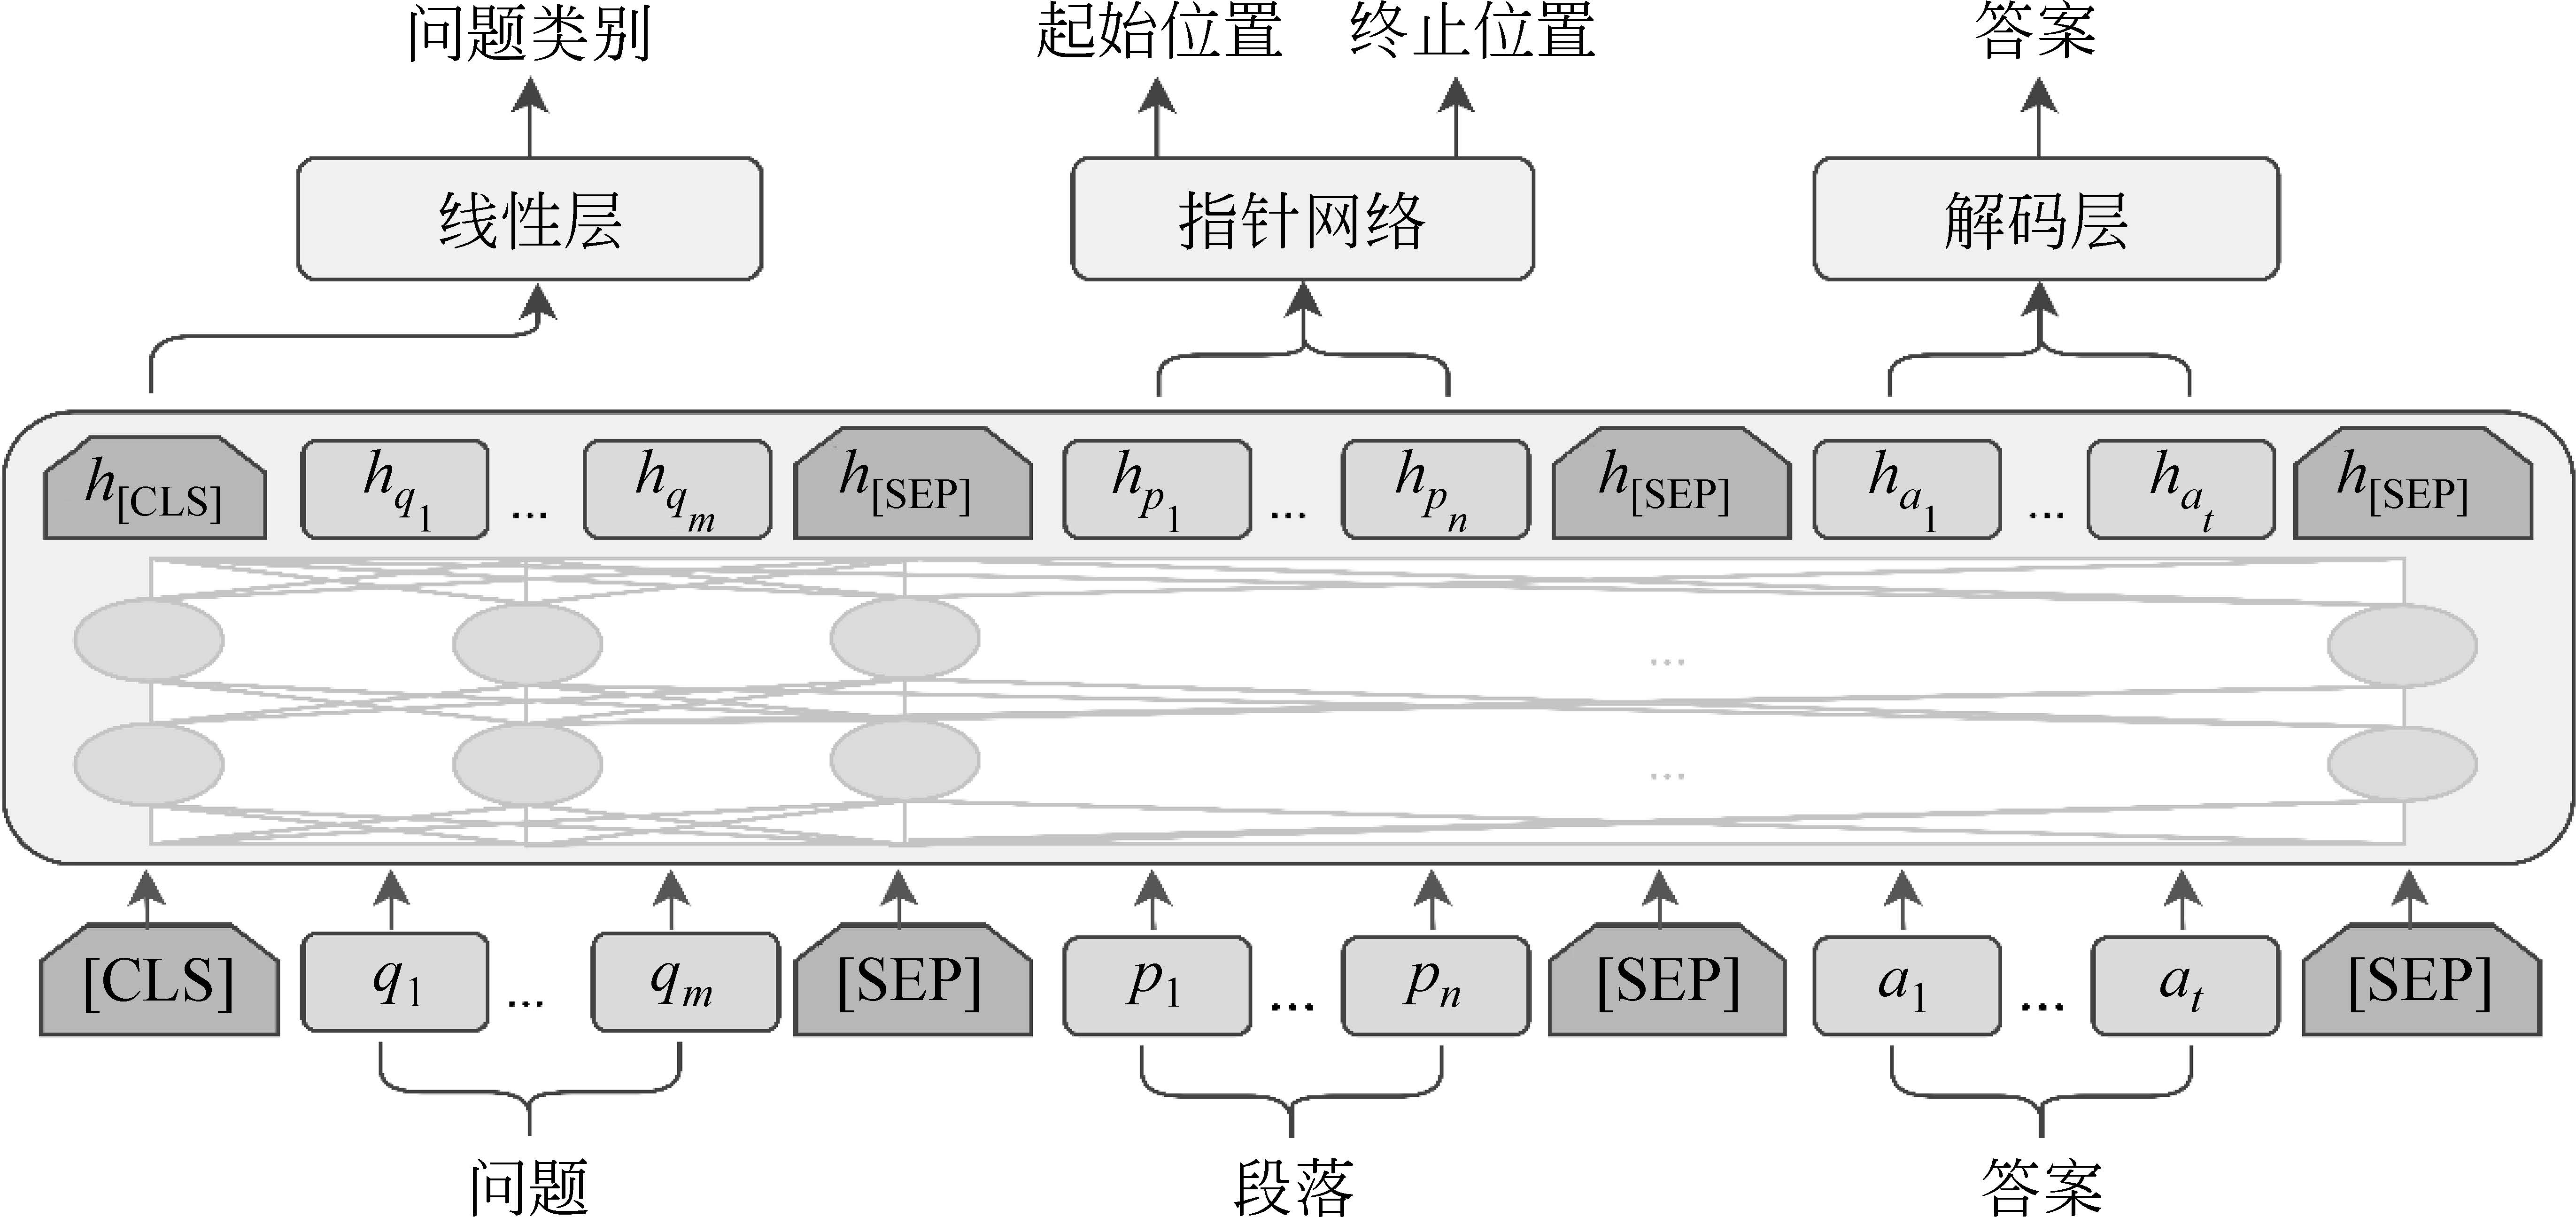
\includegraphics{./fig/model.jpg}
    \end{figure}

    任务层由答案生成模型、答案抽取模型和问题分类模型三部分组成

\end{frame}

\begin{frame}
    \frametitle{任务层}

    答案生成模型:

    \begin{itemize}
        \item 训练阶段:
        \begin{itemize}
            \item 真实答案会以一定概率被随机遮蔽
            \item 通过解码层对被遮蔽的词项进行预测来生成答案
        \end{itemize}

        \begin{equation}
            H^a = LayerNorm(Gelu(Linear(H^a)))
        \end{equation}
    
        \begin{equation}
            \alpha = Softmax(Linear(H^a))
        \end{equation}

        \item 测试阶段:直接采用训练好的解码层和beam search对问题和段落进行解码,生成答案
    \end{itemize}

    答案抽取模型:通过指针网络对答案的起始和终止位置进行识别

    \begin{equation}
        s, e = Softmax(Linear(H^p))
    \end{equation}

    问题分类模型:用线性层判断问题的类别

    \begin{equation}
        c = Softmax(Linear(H^{cls}))
    \end{equation}
\end{frame}

\subsection{论文总结}
\begin{frame}
    \frametitle{论文总结}

    \begin{itemize}
        \item 针对问题:生成式阅读理解模型缺乏答案边界和问题分类信息的理解
        \item 提出模型:基于多任务学习的生成式阅读理解模型,通过答案抽取模型和问题分类模型优化生成式阅读理解模型
        \item 实验结果:在CoQA,MS MARCO(NLG),NarrativeQA三个数据集上均取得目前生成式模型的最好性能
    \end{itemize}

\end{frame}

\section{Baseline}
\begin{frame}
    \frametitle{Baseline}

    没有细看,仅初步浏览

    模型:UniLM,与上篇论文中的baseline相似

    \begin{figure}
        \centering
        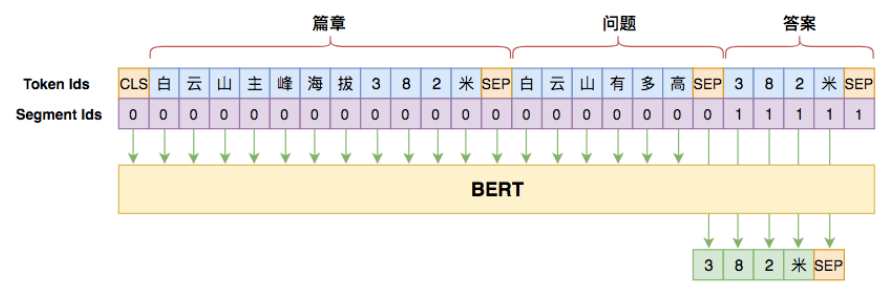
\includegraphics[scale=0.4]{./fig/baseline.png}
    \end{figure}

    输出处理:普通的beam search基础上加上按篇章平均

    存在问题:模型缺乏答案边界和问题分类信息的理解

    解决方法:使用多任务学习进行优化

\end{frame}

\section{数据集}
\begin{frame}
    \frametitle{数据集}

    仅初步了解

    \begin{itemize}
        \item CoQA:基于多个领域的多轮对话进行构建,保持了人类对话简短的特征,存在大量的指代和省略现象,问题和答案普遍较短
        \item MS MARCO:多文档问答数据集,其中提供了一个自然语言生成(NLG)的子数据集,答案并非严格匹配文档中的片段
        \item NarrativeQA:基于书本故事和电影脚本人工编辑构建的生成式阅读数据集
    \end{itemize}

\end{frame}

\section{总结}
\begin{frame}
    \frametitle{总结}

    这两天的工作:

    \begin{itemize}
        \item 阅读论文:基于多任务学习的生成式阅读理解
        \item 初步了解baseline,还未细看
        \item 初步了解相关数据集
    \end{itemize}

\end{frame}

% \begin{frame}[allowframebreaks]{References}
\begin{frame}{References}

    \nocite{*}
    \bibliographystyle{unsrt}
    \bibliography{reference.bib}

\end{frame}
\end{document}